\section{Estimation of the Warfarin Dose}

\textbf{Warfarin}

Warfarin is the most widely used oral blood anticoagulant agent worldwide;
with more than 30 million prescriptions for this drug in the United States in 2004.
The appropriate dose of warfarin is difficult to establish because it can vary substantially among patients,
and the consequences of taking an incorrect dose can be severe.  If a patient receives a dosage that is too high, they may experience excessive anti-coagulation (which can lead to dangerous bleeding), and if a patient receives a dosage which is too low, they may experience inadequate anti-coagulation (which can mean that it is not helping to prevent blood clots). Because incorrect doses contribute to a high rate of adverse effects, there is interest in developing improved strategies for determining the appropriate dose (see \href{https://www.nejm.org/doi/full/10.1056/nejmoa0809329}{paper} for further details).

\noindent Commonly used approaches to prescribe the initial warfarin dosage are the \textit{pharmacogenetic algorithm} developed by the IWPC (International Warfarin Pharmacogenetics Consortium), the \textit{clinical algorithm} and a \textit{fixed-dose} approach.

\noindent In practice a patient is typically prescribed an initial dose, the doctor then monitors how the patient responds to the dosage, and then adjusts the patient's dosage. This interaction can proceed for several rounds before the best dosage is identified. However, it is best if the correct dosage can be initially prescribed.

\noindent This question is motivated by the challenge of Warfarin dosing, and considers a simplification of this
important problem, using real data.  The goal of this question is to explore the performance of multi-armed bandit algorithms to best predict the correct dosage of Warfarin for a patient \emph{without} a trial-an-error procedure as typically employed. \\ %The algorithm will learn how to correct its prediction based on the observed response.

\textbf{Problem setting}

Let $T$ be the number of time steps. At each time step $t$, a new patient arrives and we
observe its individual feature vector $X_t \in \mathbb{R}^d$: this represents the available knowledge about the patient (e.g., gender, age, \dots).  The decision-maker (your algorithm) has access to $K$ arms, where the arm represents the warfarin dosage to provide to the patient.
For simplicity, we discretize the actions into $K=3$
\begin{itemize}
    \item Low warfarin dose: under 21mg/week
    \item Medium warfarin dose: 21-49 mg/week
    \item High warfarin dose: above 49mg/week
\end{itemize}
If the algorithm identifies the correct dosage for the patient, the reward is 0, otherwise a reward of $-1$ is received.


\noindent Lattimore and Szepesvári have a nice series of blog posts that provide a good introduction to bandit algorithms, available here:  \href{http://banditalgs.com}{BanditAlgs.com}. The \href{http://banditalgs.com/2016/09/04/bandits-a-new-beginning/}{Introduction} and the \href{http://banditalgs.com/2016/10/19/stochastic-linear-bandits/}{Linear Bandit} posts may be particularly of interest. For more details of the available Bandit literature you can check out the \href{https://tor-lattimore.com/downloads/book/book.pdf}{Bandit Algorithms Book} by the same authors. \\


\textbf{Dataset}

We use a publicly available patient dataset that was collected by staff at the Pharmacogenetics and Pharmacogenomics Knowledge Base (PharmGKB) for 5700 patients who were treated with warfarin from 21 research groups spanning 9 countries and 4 continents. You can find the data in \texttt{warfarin.csv} and metadata containing a description of each column in \texttt{metadata.xls}. Features of each patient in this dataset includes, demographics (gender, race, \dots), background (height, weight, medical history, \dots), phenotypes and genotypes.

\noindent Importantly, this data contains the true patient-specific optimal warfarin doses (which are initially unknown but are eventually found through the physician-guided dose adjustment process over the course of a few weeks) for 5528 patients. You may find this data in mg/week in \texttt{Therapeutic Dose of Warfarin}\footnote{You cannot use \texttt{Therapeutic Dose of Warfarin} data as an input to your algorithm. } column in \texttt{warfarin.csv}. There are in total 5528 patient with known therapeutic dose of warfarin in the dataset (you may drop and ignore the remaining 173 patients for the purpose of this question). Given this data you can classify the right dosage for each patient as \textit{low}: less than 21 mg/week, \textit{medium}: 21-49 mg/week and \textit{high}: more than 49 mg/week, as defined in \href{https://www.nejm.org/doi/full/10.1056/nejmoa0809329}{paper} and our Problem Setting section.

\noindent \textit{Note: the data processing steps are already implemented for you in ~utils/data_preprocessing.py~}


\begin{enumerate}[(a)]

	\input{01-estimation-warfarin-dose/01-baseline-implementation}

	\item \points{1b}

Please implement the Disjoint Linear Upper Confidence Bound (LinUCB) algorithm from \href{https://arxiv.org/pdf/1003.0146.pdf}{paper} in ~submission.py~. Below we have provided a snippet of Algorithm 1 from the listed paper. For a thorough description of terms please read through the paper.

\begin{figure}[H]
\centering
  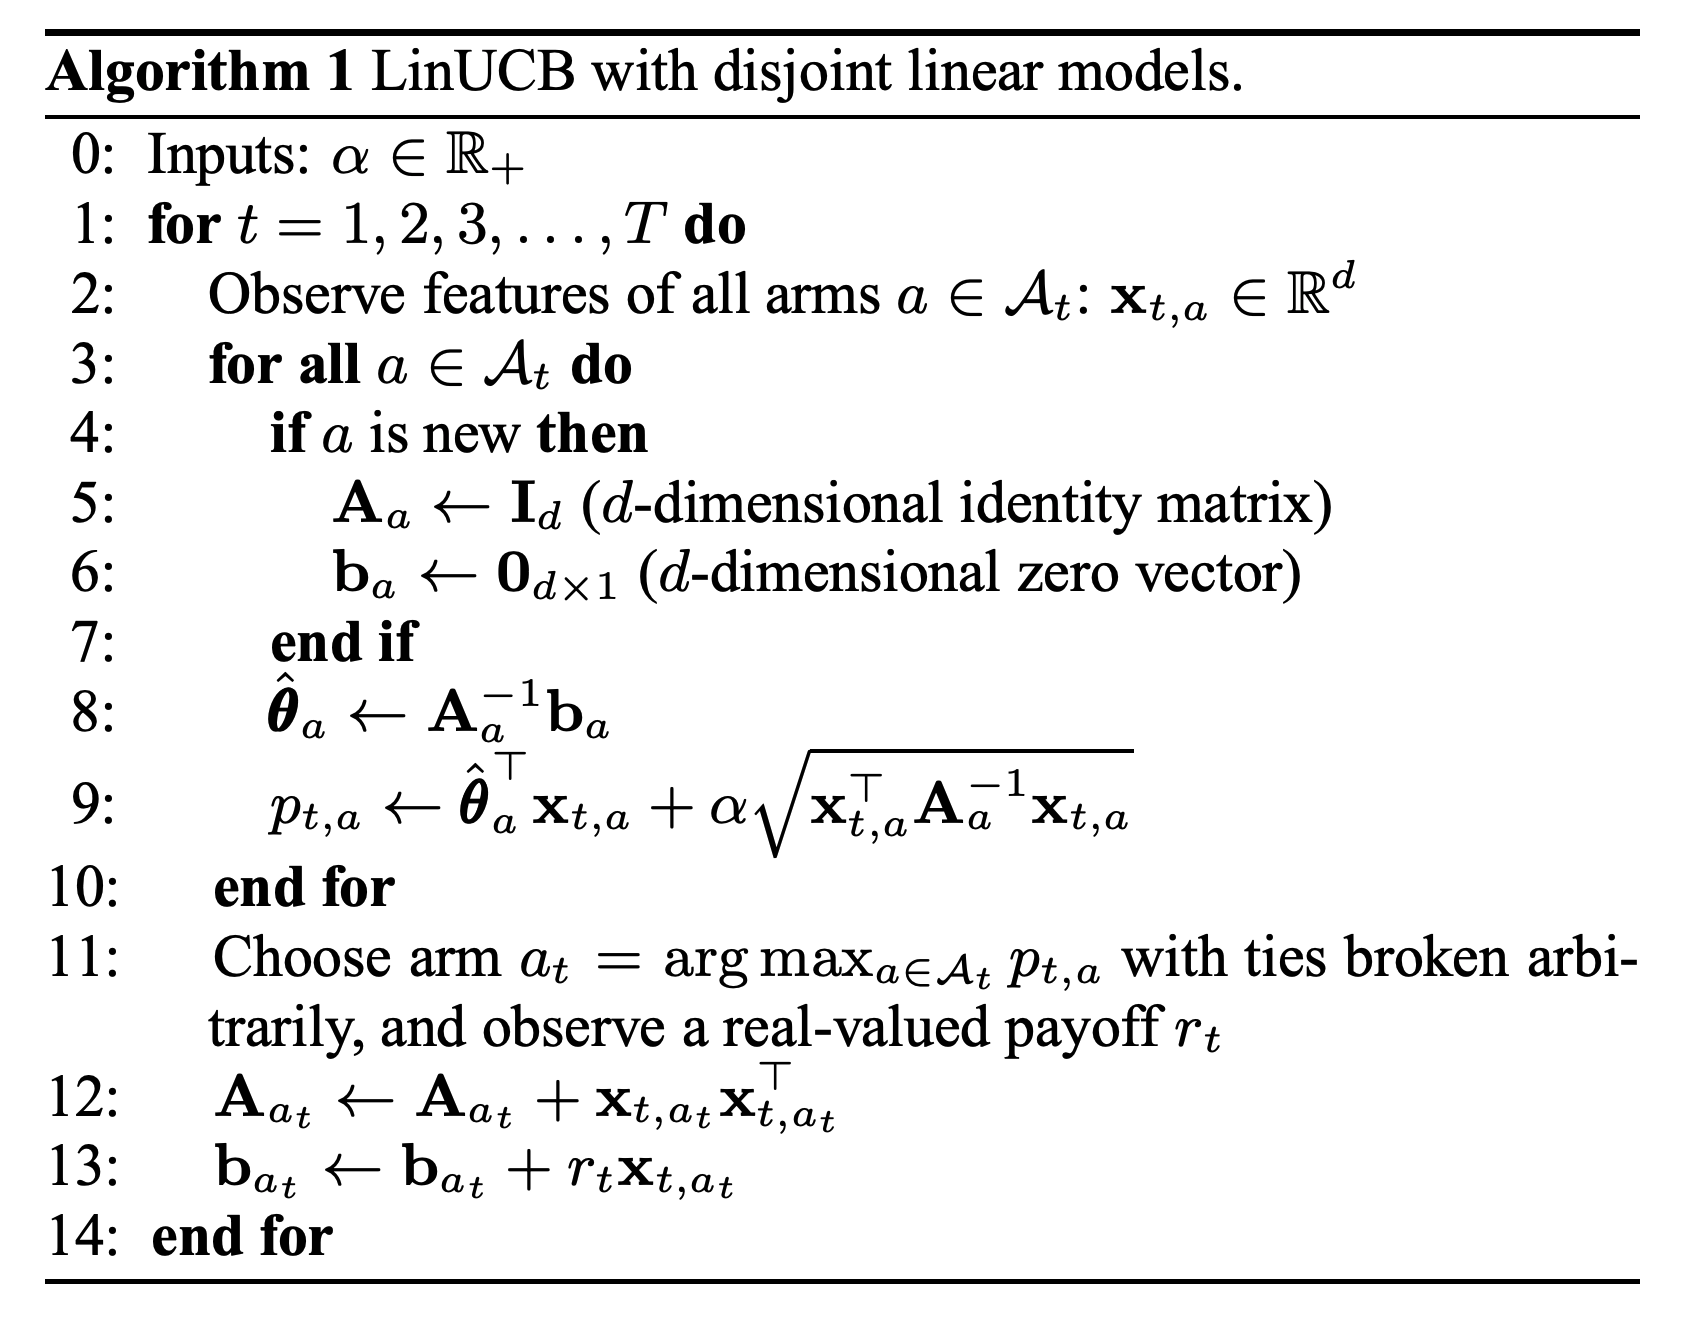
\includegraphics[width=.5\linewidth]{images/linucb_algorithm.png}
  \caption{Definition of the disjoint linear UCB algorithm taken from \href{https://arxiv.org/pdf/1003.0146.pdf}{paper}}
\end{figure}

Run the LinUCB algorithm with the following command:

\begin{lstlisting}
$ python run.py --model linucb
\end{lstlisting}

You should see the total\_fraction\_correct to be above 0.64, though the results may vary per run.

\textit{Note 1: please feel free to adjust the --alpha argument, but you don't have to.}

\textit{Note 2: for arbitrary tie breaking in action selection please simply use ~np.argmax()~.}


	\item \points{1c}

Is the upper confidence bound making a difference? Please implement the e-Greedy algorithm in ~submission.py~. Does eGreedy perform better or worse than Upper Confidence bound? (You do not need to include your answers here). 

Run the $\epsilon$-greedy LinUCB with the following command:

\begin{lstlisting}
$ python run.py --model egreedy
\end{lstlisting}

You should see the total\_fraction\_correct to be above 0.61, though the results may vary per run.

\textit{Note: please feel free to adjust the --ep argument, but you don't have to.}

	\item \points{1d}

Please implement the Thompson Sampling for Contextual Bandits from  \href{http://proceedings.mlr.press/v28/agrawal13.pdf}{paper} in ~submission.py~. Below we have provided a snippet of Algorithm 1 from section 2.2 of the listed paper. For a thorough description of terms please read through the paper.

\begin{figure}[H]
\centering
  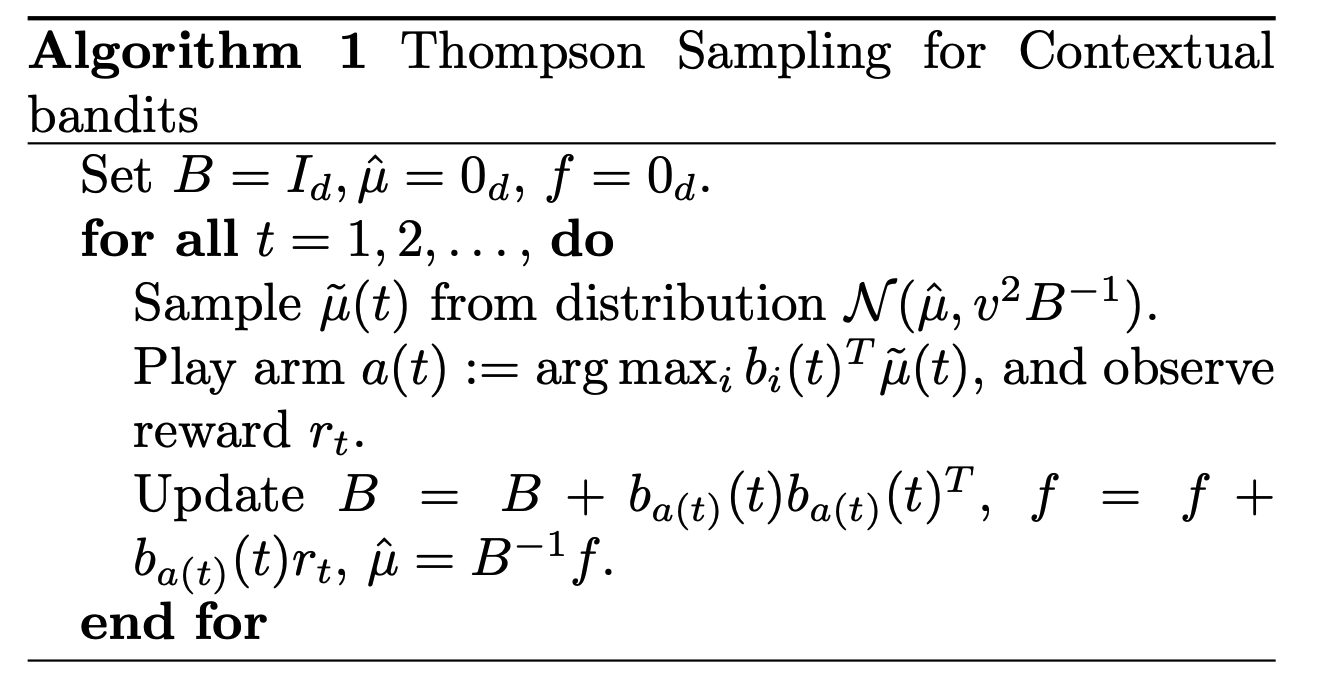
\includegraphics[width=.5\linewidth]{images/thompson_sampling_algorithm.png}
  \caption{Definition of the Thompson sampling algorithm taken from \href{http://proceedings.mlr.press/v28/agrawal13.pdf}{paper}}
\end{figure}

Run the Thompson Sampling algorithm with the following command:

\begin{lstlisting}
$ python run.py --model thompson
\end{lstlisting}

You should see the total\_fraction\_correct to be \textbf{around} 0.64, though the results may vary per run.

\textit{Note: please feel free to adjust the --v2 argument, but you don't have to. This is actually v squared from the paper) }

\end{enumerate}

\textbf{Results}

At this point, you should see a plot in your results folder titled ~fraction_incorrect.png~. If not, run the following command to generate the plot:
\begin{lstlisting}
$ python run.py
\end{lstlisting}
This will only work given you have populated csv files for each model in the results folder (e.g. ~Fixed.csv~). If you are missing a model's csv file please run the given model once more (as we have outlined in previous questions) to regenerate a csv.

You can expect your results to resemble the plot on the following page.
\begin{figure}[H]
\centering
  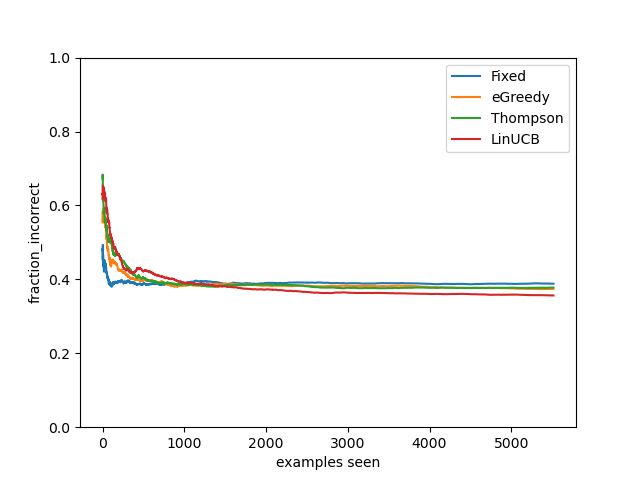
\includegraphics[width=.5\linewidth]{images/fraction_incorrect.png}
  \caption{Sample results for the correct implementation of all models.}
\end{figure}

\clearpage
